\begin{figure}[htbp]

\centering

\begin{subfigure}[t]{0.49\textwidth}
\captionsetup{labelformat=empty}

\caption{\textbf{AAPL}}
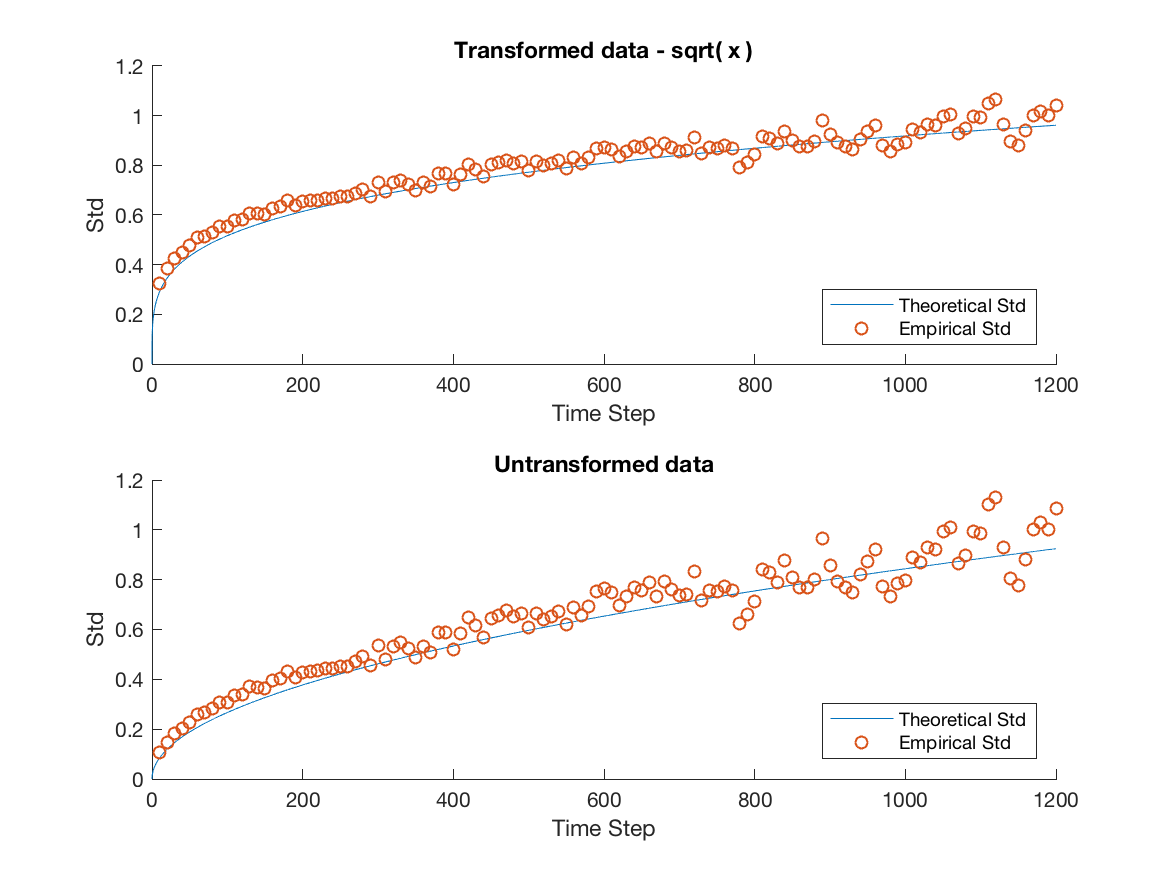
\includegraphics[width=\textwidth]{2SDO_Fit/AAPL_Plot_GCHP2SDO_21600.png}

\end{subfigure}
\begin{subfigure}[t]{0.49\textwidth}
\captionsetup{labelformat=empty}

\caption{\textbf{AMZN}}
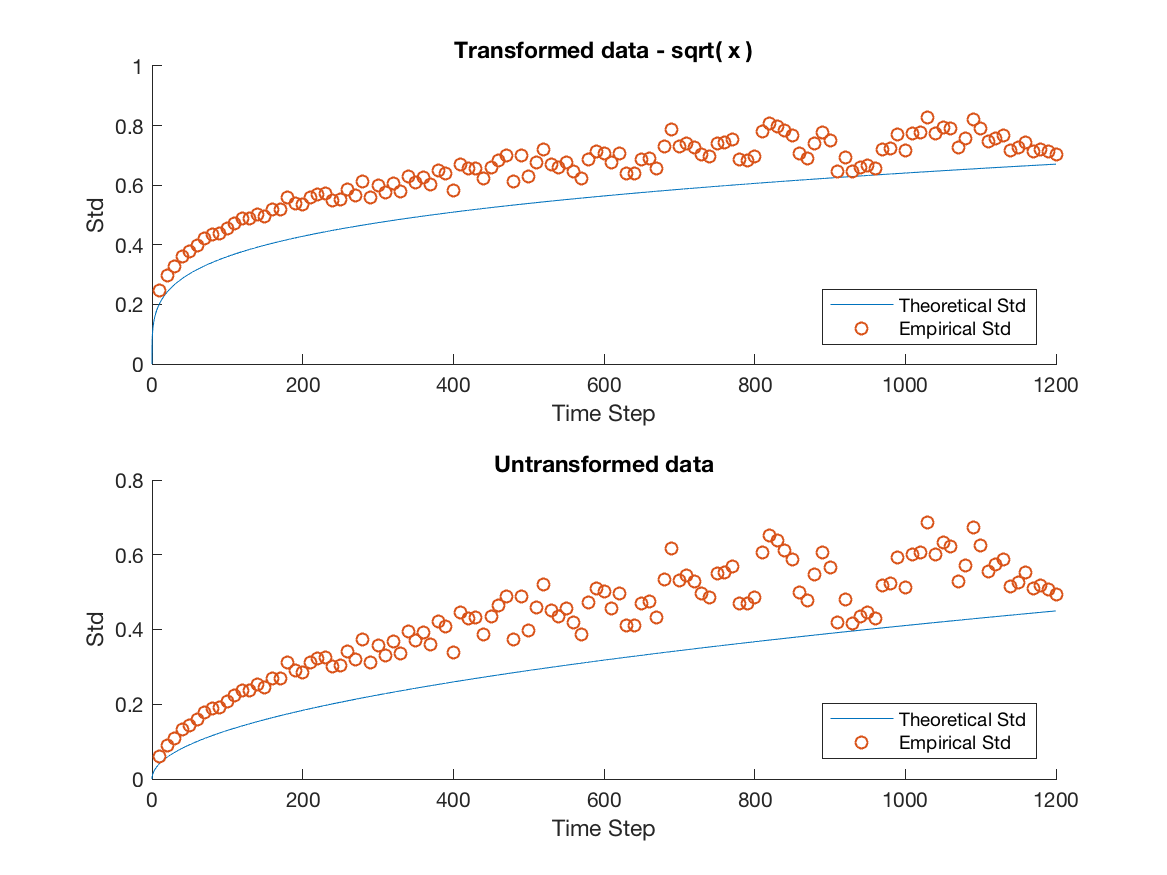
\includegraphics[width=\textwidth]{2SDO_Fit/AMZN_Plot_GCHP2SDO_21600.png}

\end{subfigure}

\begin{subfigure}[t]{0.49\textwidth}
\captionsetup{labelformat=empty}

\caption{\textbf{GOOG}}
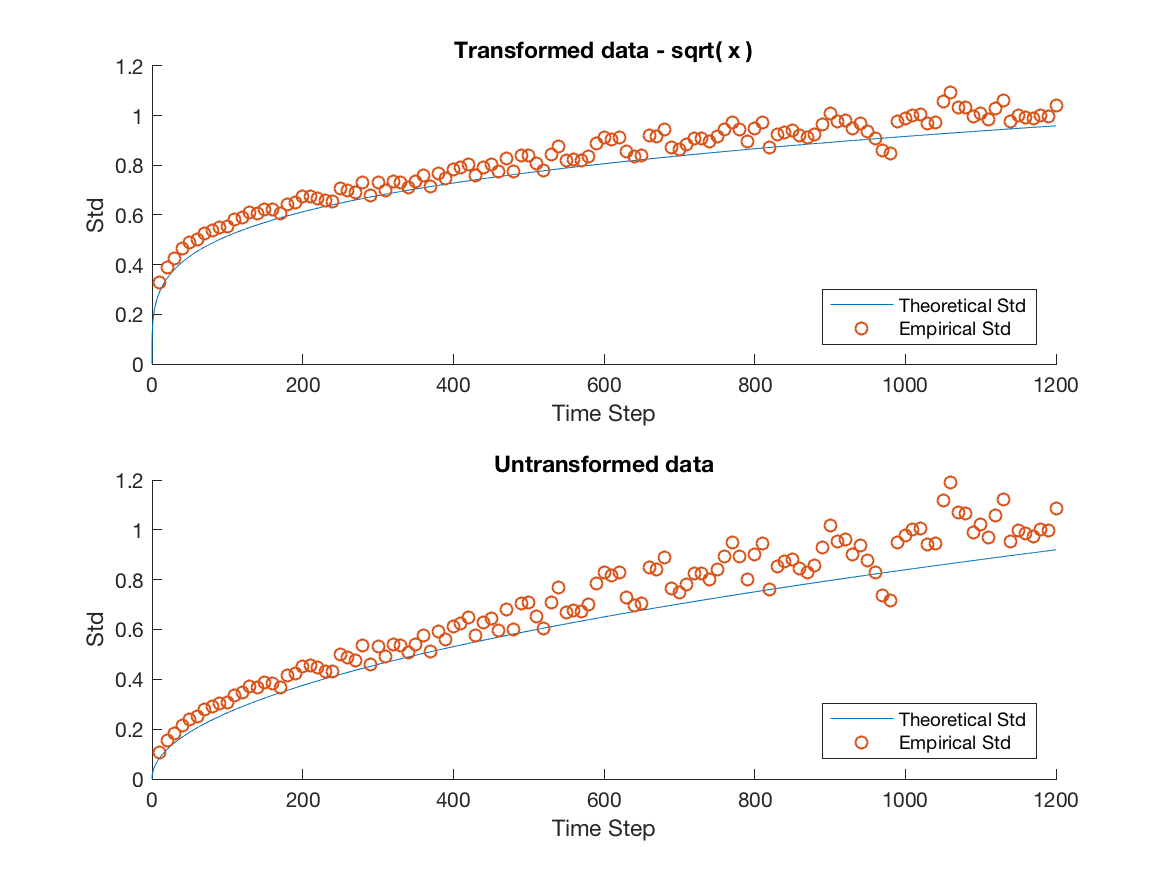
\includegraphics[width=\textwidth]{2SDO_Fit/GOOG_Plot_GCHP2SDO_21600.png}

\end{subfigure}

\caption{\label{fig:2SDOfit} A comparison of the empirical standard deviation for a fixed window size $n$ to the theoretical standard deviation for AAPL, AMZN and GOOG using the 2 state dependent order model. We have plotted the empirical standard deviation for all $n$ from 10 seconds to 20 minutes in step sizes of 10 seconds. Each empirical standard deviation corresponds to a single point in the scatter plot and the plotted curve corresponds to the predicted theoretical value. Visually there is a significant improvement for all stocks, although the theoretical standard deviation for AMZN is still underestimating the empirical variability.}

\end{figure}